\documentclass[a4paper,10pt]{article}
\usepackage{geometry}
\usepackage{mathtools}
\usepackage{amsfonts}
\usepackage{amsmath}
\usepackage[utf8]{inputenc}

 \geometry{
 a4paper,
 total={170mm,257mm},
 left=20mm,
 top=30mm,
 }
\usepackage{fancyhdr}
\fancyhead[L]{Leonard Korp 302582 \\ Nikita Malyschkin 319500 \\ Valentin Engelke 358096}
\fancyhead[R]{WS 2017/18 \\ 16.11.2017}
\pagestyle{fancy}



\begin{document}
\centerline{\Large\bfseries  Foundations of Data Science }
\centerline{\bfseries  Exercise sheet 6}
\section*{Exercise 1}
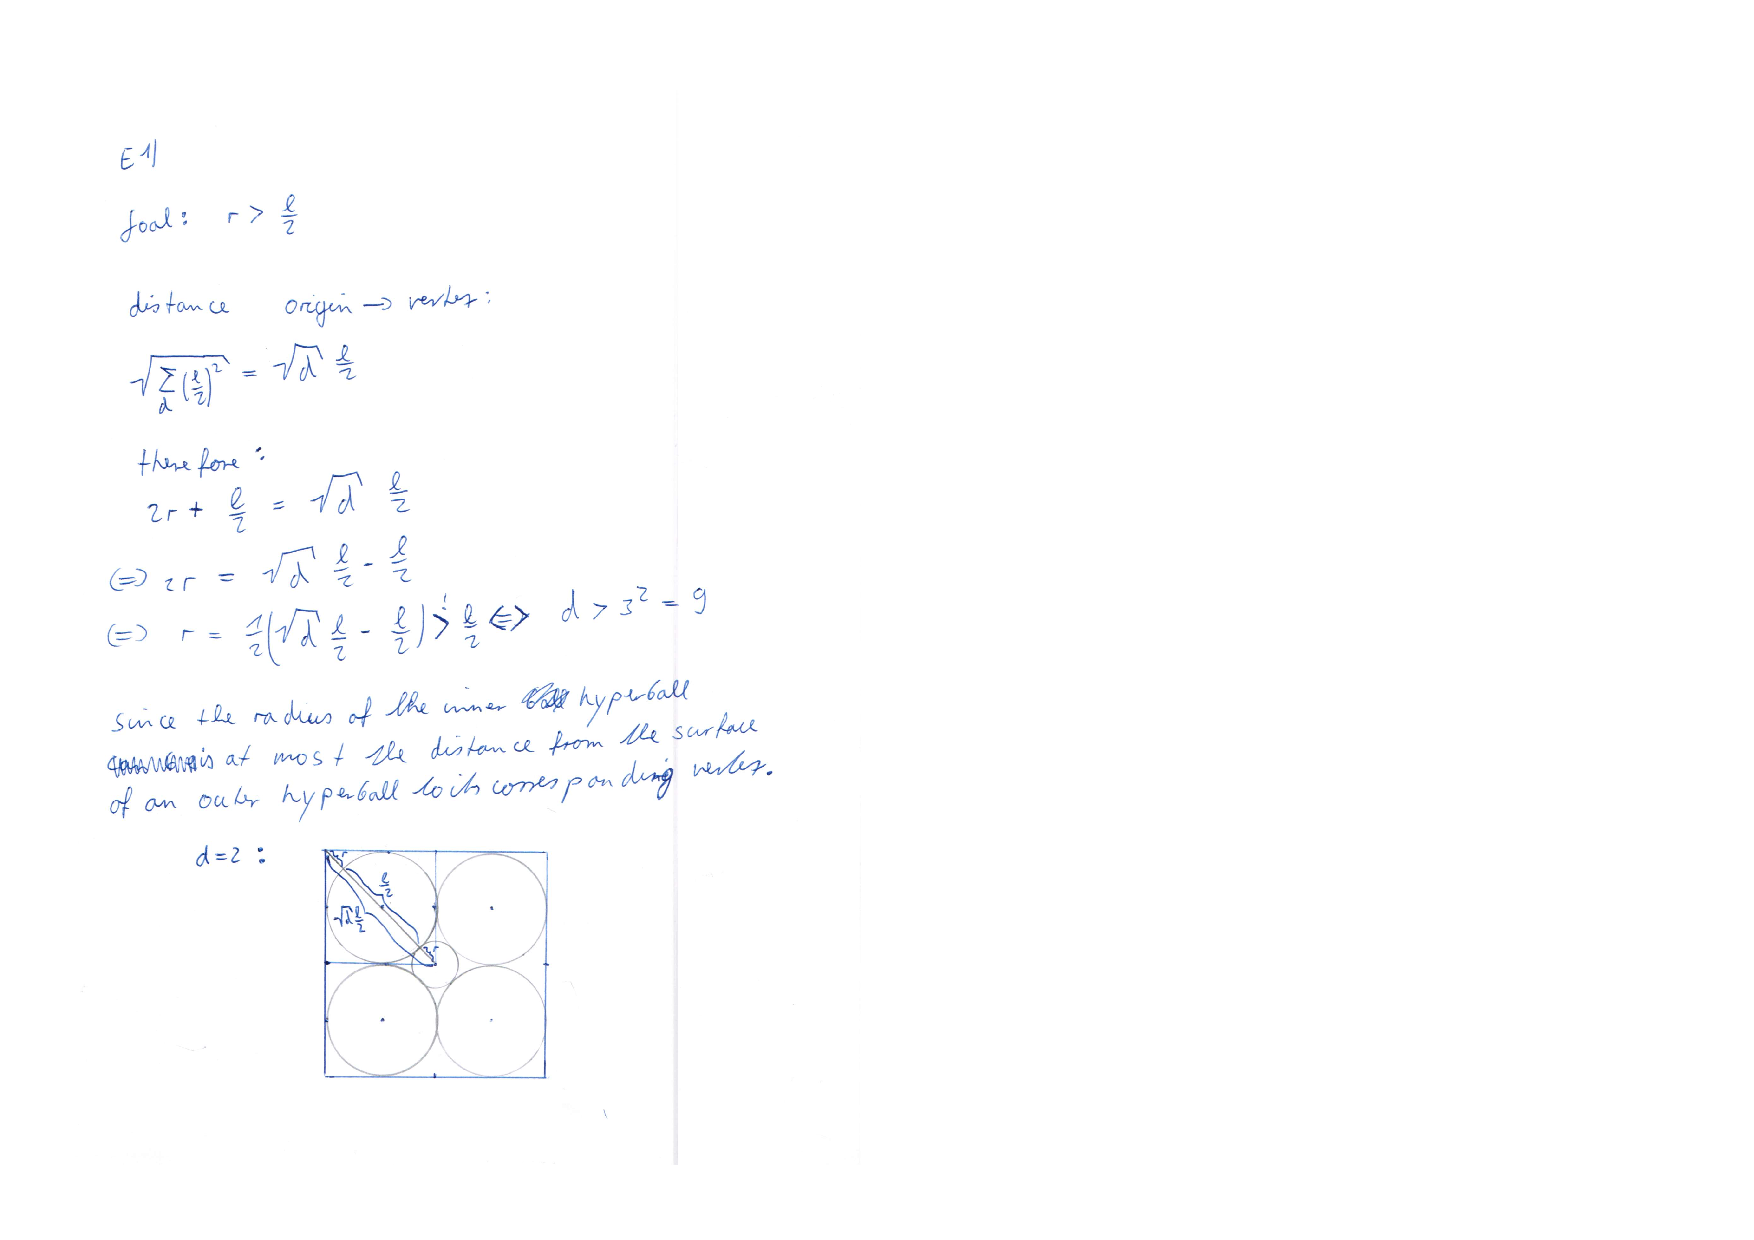
\includegraphics[scale=1]{E1.pdf}
\section*{Exercise 2}
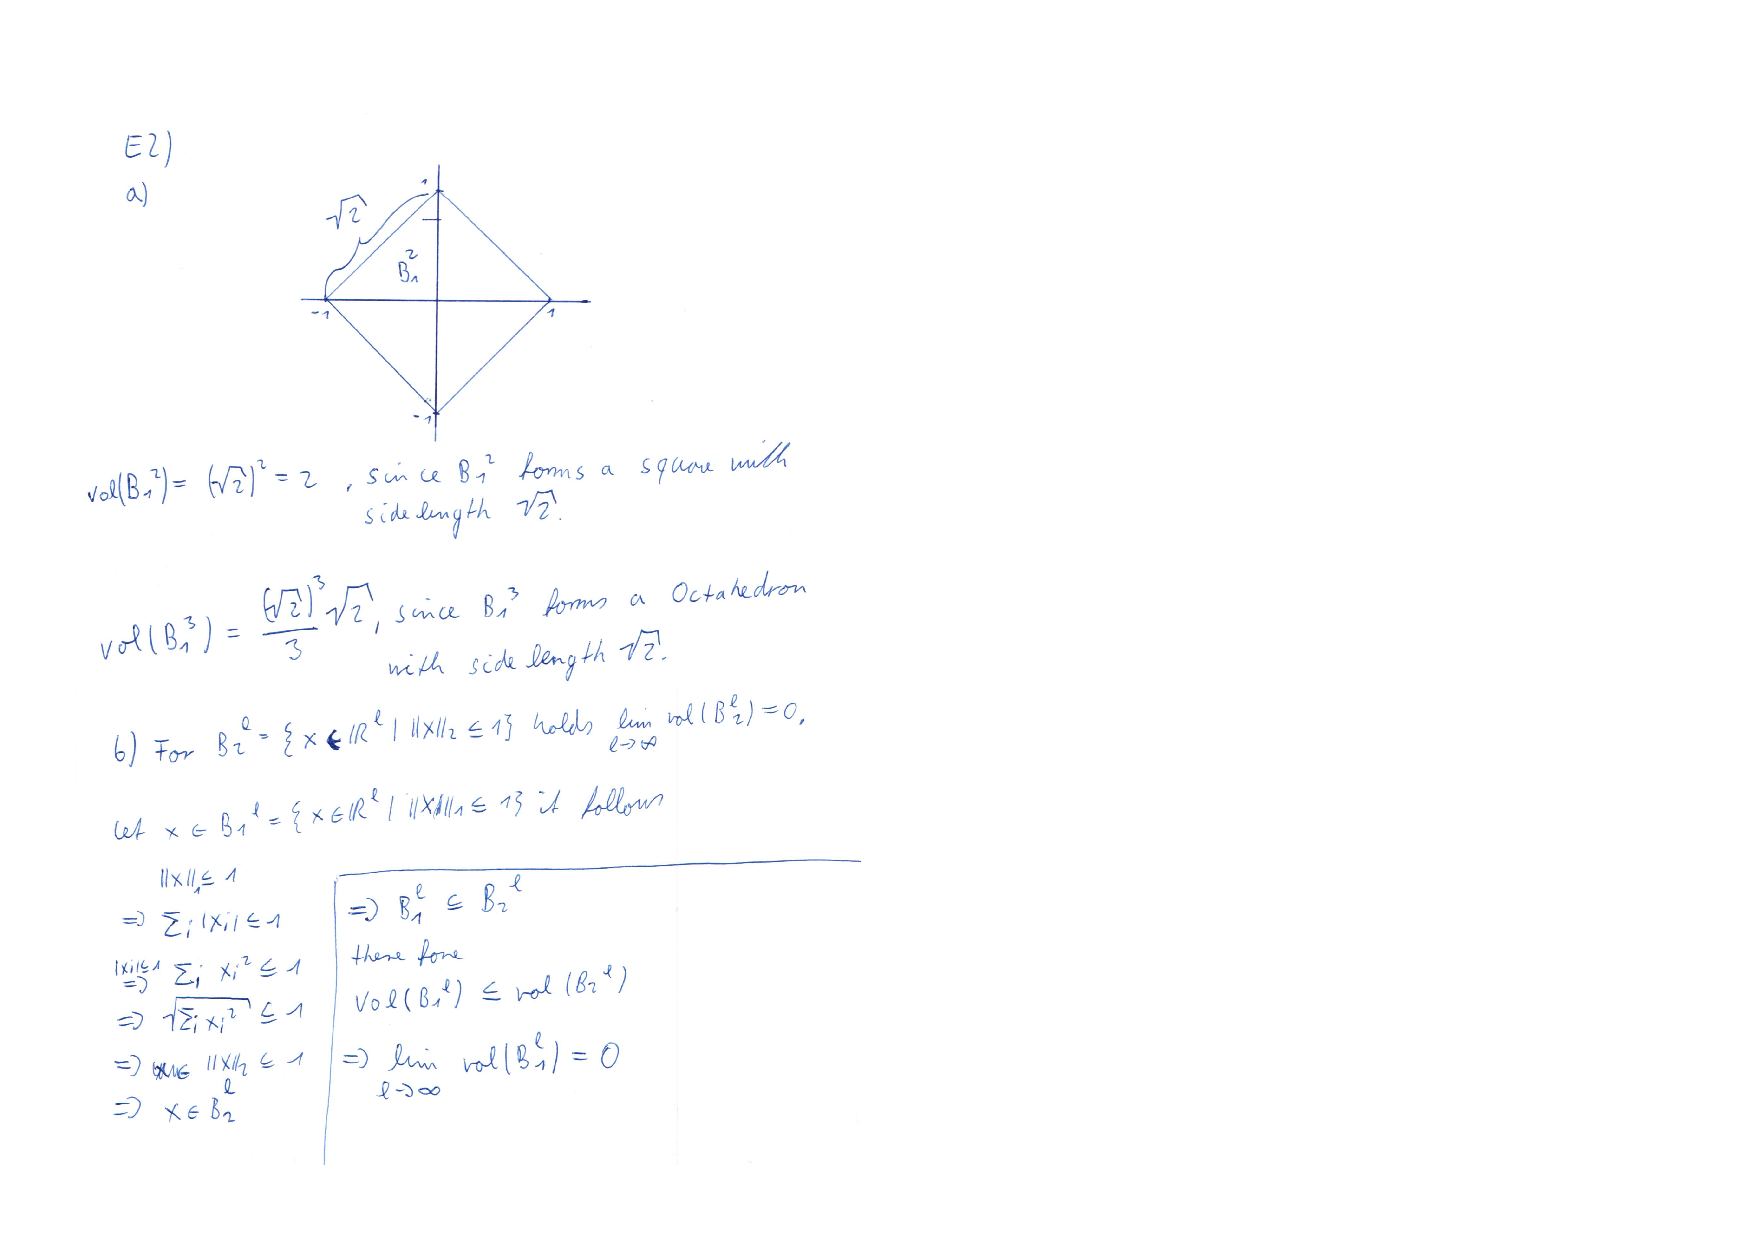
\includegraphics[scale=1]{E2.pdf}

\section*{Exercise 3}
\subsection*{a)}

\[M^TM = \left( \begin{array}{ccccc}
1 & 3 & 5 & 0 & 1 \\
2 & 4 & 4 & 2 & 3 \\
3 & 5 & 3 & 4 & 5 \\
\end{array} \right)
%
\left( \begin{array}{ccccc}
1 & 2 & 3 \\
3 & 4 & 5 \\
5 & 4 & 3 \\
0 & 2 & 4 \\
1 & 3 & 5 \\
\end{array} \right)
=\left( \begin{array}{ccc}
36 & 37 & 38 \\
37 & 49 & 61 \\
38 & 61 & 84 \\
\end{array} \right)
\]
\[MM^T = 
\left( \begin{array}{ccccc}
1 & 2 & 3 \\
3 & 4 & 5 \\
5 & 4 & 3 \\
0 & 2 & 4 \\
1 & 3 & 5 \\
\end{array} \right) 
\left( \begin{array}{ccccc}
1 & 3 & 5 & 0 & 1 \\
2 & 4 & 4 & 2 & 3 \\
3 & 5 & 3 & 4 & 5 \\
\end{array} \right)
=
\left( \begin{array}{ccccc}
14 & 26 & 22 & 16 & 22 \\
26 & 50 & 46 & 28 & 40 \\
22 & 46 & 50 & 20 & 32 \\
16 & 28 & 20 & 20 & 26 \\
22 & 40 & 32 & 26 & 35 \\
\end{array} \right)
\]

\subsection*{b)}
$ det(M^TM-\lambda I) = -\lambda^3 +169 \lambda^2 -2370 = -\lambda * (\lambda^2-169 \lambda +2370) =0 $ \\
$\lambda_1 =0 \ \ \lambda_{2,3}=\frac{169}{2} \pm \sqrt{\frac{19081}{4}}$ \\\\

$ det(MM^T-\lambda I) = -\lambda^5+169\lambda^4-2370\lambda^3 = -\lambda^3 * (\lambda^2-169 \lambda +2370) =0 $ \\
$\lambda_{1,2,3} =0 \ \ \lambda_{4,5}=\frac{169}{2} \pm \sqrt{\frac{19081}{4}}$
 \subsection*{c)}
 $ (M^TM-\lambda I)*x = 0 $ \\
 $\lambda_1=0$
 \[\left( \begin{array}{ccc|c}
36 & 37 & 38 & 0\\
37 & 49 & 61 & 0\\
38 & 61 & 84 & 0\\
\end{array} \right) \rightarrow  \left( \begin{array}{ccc|c}
36 & 37 & 38 & 0\\
0 & 395 & 790 & 0\\
0 & 395 & 790 & 0\\
\end{array} \right) \]\\
$x_3 = -2x_2 \Rightarrow x_1=x_3 \Rightarrow x= \left(
\begin{array}{c}
1\\
-2\\
1\\
\end{array}
\right) $ \\ \\
 $\lambda_2=\frac{169}{2} - \sqrt{\frac{19081}{4}} \\
 x= \left(
\begin{array}{c}
-1.45\\
-0.22\\
1\\
\end{array}
\right) $ \\
 $\lambda_3=\frac{169}{2} + \sqrt{\frac{19081}{4}} \\
 x= \left(
\begin{array}{c}
0.57\\
0.79\\
1\\
\end{array}
\right) $ \\ \\ \\
 $ (MM^T-\lambda I)*x = 0 $ \\
$\lambda_{1,2,3}=0$%
\[\left( \begin{array}{ccccc|c}
14 & 26 & 22 & 16 & 22 & 0 \\
26 & 50 & 46 & 28 & 40 & 0\\
22 & 46 & 50 & 20 & 32 & 0\\
16 & 28 & 20 & 20 & 26 & 0\\
22 & 40 & 32 & 26 & 35 & 0\\
\end{array} \right)
\rightarrow
\left( \begin{array}{ccccc|c}
14 & 26 & 22 & 16 & 22 & 0 \\
0 & 12 & 36 & -12 & -6 & 0\\
0 & 36 & 108 & -36 & -18 & 0\\
0 & -12 & -36 & 12 & 6 & 0\\
0 & -6 & -18 & 6 & 3 & 0\\
\end{array} \right) 
 \] \\
 $x_2=r,x_3=s,x_4=t \Rightarrow x_5 =2r+6s-2t \Rightarrow x_1=2t-11s-5r$ \\
 $x=\left(
\begin{array}{c}
2t-11s-5r\\
r\\
s\\
t\\
2r+6s-2t
\end{array}
\right)$ \\
 three eigenvectors for eigenvalue 0:\\
\[ \left(
\begin{array}{c}
-5\\
1\\
0\\
0\\
2
\end{array}
\right) \ \ \left(
\begin{array}{c}
-11\\
0\\
1\\
0\\
6
\end{array}
\right) \ \ \left(
\begin{array}{c}
2\\
0\\
0\\
1\\
-2
\end{array}
\right)  \]  \\ \\
$\lambda_{4}=\frac{169}{2} - \sqrt{\frac{19081}{4}} $ \\
$x_4 =  \left(
\begin{array}{c}
0.38\\
-0.08\\
-1.78\\
1.23\\
1
\end{array}
\right)$ \\ \\
$\lambda_{5}=\frac{169}{2} + \sqrt{\frac{19081}{4}} $ \\
$x_5 =  \left(
\begin{array}{c}
0.65\\
1.24\\
1.13\\
0.70\\
1
\end{array}
\right)$ \\ \\
\subsection*{d)}
$\lambda_1=\frac{169}{2} + \sqrt{\frac{19081}{4}},\lambda_2 = \frac{169}{2} - \sqrt{\frac{19081}{4}}$ \\
$\sigma_1=\sqrt{\lambda_1}=12.39$ \\
$\sigma_2=\sqrt{\lambda_2}=3.93$ \\
$u_1=\left(
\begin{array}{c}
0.57\\
0.79\\
1\\
\end{array}
\right) \\
u_2= \left(
\begin{array}{c}
-1.45\\
-0.22\\
1\\
\end{array}
\right)$
\section*{Exercise 4}

\end{document}

